\documentclass{report}

\usepackage{cmap}
\usepackage[T2A]{fontenc}
\usepackage[utf8]{luainputenc}
\usepackage[english, russian]{babel}
\usepackage[pdftex]{hyperref}
\pagestyle{plain}
\usepackage[14pt]{extsizes}
\usepackage[a4paper, mag=1000, bottom=3cm, top=2cm, left=2.5cm, right=1cm, top=2cm, bottom=2cm, headsep=0.7cm, footskip=1cm]{geometry}
\usepackage{listings}
\usepackage{indentfirst}
\usepackage{tikz}
\usepackage{color}
\usepackage[]{caption}
\usepackage{chngcntr}
\usepackage{multirow}
\usepackage{hhline}
\usepackage{multicol}
\usepackage{enumitem}










\makeatletter
\renewcommand\@biblabel[1]{#1.\hfil}
\makeatother

\setlist{nolistsep, itemsep=0.3cm,parsep=0pt}
\setlength{\parskip}{0.5cm}

\lstset{language=C++,
	basicstyle=\footnotesize\ttfamily,
	keywordstyle=\color{blue}\ttfamily,
	stringstyle=\color{red}\ttfamily,
	commentstyle=\color{green}\ttfamily,
	morecomment=[l][\color{magenta}]{\#},
	tabsize=2,
	breaklines=true,
	breakatwhitespace=true
}



\begin{document}
	\begin{titlepage}
		
		\begin{center}
			Министерство науки и высшего образования Российской Федерации
		\end{center}
		
		\begin{center}
			Федеральное государственное автономное образовательное учреждение высшего образования \\
			Национальный исследовательский Нижегородский государственный университет им. Н.И. Лобачевского
		\end{center}
		
		\begin{center}
			Институт информационных технологий, математики и механики
		\end{center}
		
		\vspace{4em}
		
		\begin{center}
			\textbf{\LargeОтчет по лабораторной работе} \\
		\end{center}
		\begin{center}
			\textbf{\Large«Умножение разреженных матриц. Элементы комплексного типа. Формат хранения матрицы – столбцовый (CCS)»} \\
		\end{center}
		
		\vspace{11em}
		\hfill\parbox{6.5cm}{
			\textbf{Выполнил:} \\ студент группы 381708-1 \\ Шеметов Ф.А.\\
			\\
			\textbf{Проверил:}\\ доцент кафедры МОСТ, \\ кандидат технических наук \\ Сысоев А. В.
		}
		
		\vspace{\fill}
		\begin{center} Нижний Новгород \\ 2020 \end{center}
		
	\end{titlepage}
	
	\setcounter{page}{2}
	
	\tableofcontents
	\newpage
	
	\section*{Введение}
	\addcontentsline{toc}{section}{Введение}
	
	Разрежённой матрицей называются матрицы, которые преимущественно состоят из нулевых элементов. Возникают разрежённые матрицы при решении различных задач связанных с научной и инженерной областью, где присутствует большое число неизвестных, связанных между собой уравнениями.
	\par Так как в разрежённых матрицах содержится большинство значений в виде нулей, то любая арифметическая операция с этими матрицами увеличивает лишние вычислительные затраты. Для того чтобы снизить вычислительные затраты, были придуманы разные способы хранений разрежённых матриц и один из них --- Формат хранения CCS\footnote{Compressed Column Storage}. 
	\par Формат хранения CCS представляет собой структуру данных, которая позволяет хранить матрицу в виде трех массивов. Первый массив хранит ненулевые значения элементов матрицы. Второй массив хранит номера строк для каждого ненулевого элемента. Третий массив хранит индекс начала каждого столбца.
	\par Сам формат хранения CCS предоставляет минимальные требования к памяти и значительно уменьшает вычислительные затраты при арифметических операциях с разрежёнными матрицами.
	\par Цель лабораторной работы --- изучение принципа хранения и разработка алгоритма умножения разрежённых матриц в формате CCS с использованием технологий параллельного программирования.
	\newpage
	
	\section*{Постановка задачи}
	\addcontentsline{toc}{section}{Постановка задачи}
	В данной лабораторной работе ставится задача в виде разработки нескольких проектов, где нужно реализовать алгоритм умножения разрежённых матриц в формате хранения CCS с элементами комплексного типа.
	\par Проект будет включать в себя:
	\begin{itemize}
		\item Набор юнит-тестов использующие Google C++ Testing Framework.
		\item Исходный и заголовочный файл. В заголовочном файле реализован интерфейс класса, а в самом исходном файле реализован код последовательного алгоритма умножения разрежённых матриц в формате хранения CCS или параллельный алгоритм с технологиями OpenMP, TBB, std::threads.
		\item файл CMake для сборки проекта.
	\end{itemize}
	\newpage
	
	
	\section*{Описание алгоритма}
	\addcontentsline{toc}{section}{Описание алгоритма}
	В нашей лабораторной работе нужно реализовать алгоритм умножения разрежённых матриц в формате хранения CCS с элементами комплексного типа.
	\parЧтобы реализовать алгоритм умножения, нужно сгенерировать саму разрежённую матрицу. Для этого мы будем использовать ГПСЧ \textit{mt19937}, который позволяет генерировать оптимально-хорошую последовательность случайных чисел. Так как мы реализовываем не плотную, а разрежённую матрицу которая преимущественно состоит из нулей, то для ГПСЧ создаём условие в виде вещественного числа от 0 до 1. Число 0 представляет собой 0\% шанс, что случайное значение будет равен 0, а 1 представляет 100\% шанс, что случайное значение будет равно нулю. И, чтоб получить разрежённую матрицу, мы указываем вещественное число больше 0.5 для получения преимущественно нулей. 
	\parПосле полученного сгенерированного класса разрежённой матрицы, нам нужно реализовать хранение этой матрицы в формате CCS. Но так как перенос из разрежённой матрицы в формат хранения CCS увеличивает вычислительные затраты, то для их уменьшения, мы сначала должны транспонировать матрицу и перевести в формат хранения CRS, получая формат хранения CCS, но возникает проблема в том, что разрежённая матрица может быть больших размеров, где большинство значений это нули, поэтому транспонирование этой матрицы будет тоже для нас затратным делом. И, чтобы снизить затраты, нужен алгоритм транспонирования, который сразу преобразует матрицу из формата хранения CRS в формат хранения CCS.
	\parПоэтому, первым делом мы преобразуем разрежённую матрицу в CRS формат. Все ненулевые значения, обходя последовательно по строкам матрицы, передаём в первый вектор(\verb|value|), во второй вектор(\verb|col_index|) мы передаём номера столбцов ненулевых значений матрицы, в третий вектор(\verb|row_offset|) передаём индексы начала новых строк во втором векторе. Получив объект класса разрежённой матрицы в формате CRS, следующий шаг это алгоритм транспонирования CRS в CCS. Сформируем новый объект класса \verb|obj| с пустыми векторами, в первом векторе(\verb|obj.value|) также будут ненулевые значение, во втором(\verb|obj.row_index|) уже будут номера строк, а в третьем(\verb|obj.col_offset|) индексы начала новых столбцов. Сначала мы заполняем третий вектор  нулями и инкрементируем значение этого вектора, где индекс является номер столбца. Получив заполненный третий вектор, мы обращаемся к нему и получаем индекс к вектору \verb|obj.col_offset| и \verb|obj.value|, где поэтому индексу во втором векторе(\verb|obj.row_index|) в элементы передаём номера строк, а в первом(\verb|obj.value|) в элементы передаём значения элементов первого вектора формата хранения CRS.
	\parПолучив объект класса разрежённой матрицы в формате хранения CCS, мы теперь можем реализовать алгоритм умножения CCS матриц. Умножение двух CCS матриц происходит по алгоритму JKI-типа, где можно увидеть на Рис.1.
	
	
	
	\begin{figure}[htbp]
		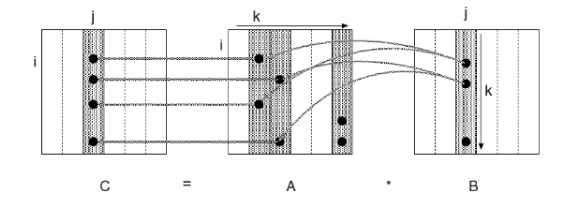
\includegraphics[width=\textwidth]{../../../../modules/reports/shemetov_p_sparse_matrix_CCS_complex/CCS_matrix.png}
		\caption{Умножение разрежённых матриц в формате хранения CCS. Постолбцовый JKI алгоритм.}
	\end{figure}
	
	
	Возьмём матрицу A и B в формате хранения CCS. Начинаем обходить столбцы матрицы B. Взяв столбец, идём по вектору \verb|col_offset| и получаем индекс расположения ненулевых элементов в строках. После чего поэтому индексу определяем номер столбца матрицы А и циклом обходим строки этого столбца, содержащие ненулевые элементы. Чтоб записывать результаты умножения, создаём новый вектор \verb|tempDataVec|, где его индекс это номер строки столбца вектора A с ненулевыми элементами. Записываем результат умножения и суммирования для каждого элемента столбца матрицы B на весь столбец матрицы А в каждый индекс вектора \verb|tempDataVec|, где заполненный вектор является столбцом исходной матрицы C. После этого, обходим циклом этот вектор, проверяем на отсутствие нулевых значений и передаём его элементы в первый вектор матрицы C, во второй, число ненулевых значений в векторе \verb|tempDataVec|, а в третий, вектор размер первого вектора. В итоге после полного выполнения алгоритма, получаем умноженную исходную матрицу C в формате CCS.
	\newpage
	
	\section*{Описание схемы распараллеливания}
	\addcontentsline{toc}{section}{Описание схемы распараллеливания}
	Параллельный алгоритм умножения можно описать следующим образом. При умножении двух матриц, последовательный код обходит все столбцы матрицы B, что затрачивает немало времени выполнения алгоритма. Используя потоки, мы распределяем каждому потоку равную часть столбцов матрицы B. Теперь каждый поток выполняет свою отдельную часть цикла обхода столбцов, умножения элементов и запись результатов, тем самым уменьшая в несколько раз время выполнения алгоритма. 
	\par При выполнении параллельного участка кода, возникает проблема в виде "Гонки Данных"{}, где два или более потока соперничают за обладанием общим ресурсом. В нашем случае это происходит, когда один поток, взявший не начальную часть цикла, выполняет быстрее участок кода, чем поток который взял часть начального цикла, из-за чего в исходные векторы матрицы C результаты потоков заполняются в неправильном порядке. Решением этой проблемы стало создание вектора векторов, то есть по сути, мы для каждого потока создали свои частный вектор с данными, куда записывают по индексу итерации результат вычислений этой итерации. Мы избавились от "Гонки Данных" и теперь спокойно можем последовательно записать в исходные векторы матрицы C частные результаты трёх векторов каждого потока. В итоге получаем матрицу C в формате CCS.
	\newpage
	
	
	\section*{Описание программной реализации}
	\addcontentsline{toc}{section}{Описание программной реализации}
	Программная реализация последовательного и параллельного алгоритма умножения представляет собой статический метод класса, который принимает два входных параметра в виде объекта класса разрежённой матрицы в формате хранения CCS. Сам вызов метода класса параллельного алгоритма умножения в коде выглядит так:
	\begin{lstlisting}
	SparseMatrixCCS SparseMatrixCCS::MultiplySparseMatrixParallel(
	const SparseMatrixCCS &A, const SparseMatrixCCS &B)
	\end{lstlisting}
	\parНазвание метода для каждой технологии параллельного программирования отличается, но остальная сигнатура метода одинакова для каждой технологии.
	
	\subsection*{OpenMP}
	\addcontentsline{toc}{subsection}{OpenMP}
	Реализация параллельного алгоритма умножения разреженных матриц с технологией OpenMP представляет собой распараллеленный цикличный обход столбцов матрицы B с помощью вызовы директивы \verb|#pragma omp parallel for|, где основной поток создает новые потоки, которые начинают выполнять свои части итераций. После выполнения всех потоков и получения локальных результатов от каждого потока, основной поток заполняет исходные вектора матрицы C значениями из локальных векторов потоков. В результате получаем разрежённую матрицу C в формате CCS.
	
	
	\subsection*{TBB}
	\addcontentsline{toc}{subsection}{TBB}
	Для реализации параллельного алгоритма умножения разреженных матриц с технологией TBB используем шаблонную функцию \verb|tbb::parallel_for()|, которая принимает несколько параметров: итерационное пространство и функтор. Итерационное пространство задается шаблонным классом \verb|tbb::blocked_range|, где входные параметры это начало и конец цикла. Сам класс позволяет рекурсивно делить итерационное пространство для каждого потока. Разделение итерационного пространства происходит автоматически планировщиком TBB.
	\parВместо функтора, можно использовать лямбда-выражение, который принимает итерационное пространство каждого потока и выполняет алгоритм умножения разрёженных матриц. После чего получаем локальные результаты от каждого потока и заполняем исходные векторы матрицы C значениями из локальных векторов потоков. 
	
	
	\subsection*{std::threads}
	\addcontentsline{toc}{subsection}{std::threads}
	В std::threads мы первым делом выделяем память под объекты \verb|std::thread|, которые являются отдельными потоками. После этого вычисляем порции итераций для каждого потока, путем деления общего числа итераций на количество потоков, а остаток от деления прибавляем к последнему потоку.
	\par В объект \verb|std::thread[i]|, где \emph{i} это поток, передаём лямбда-выражение, в который передаем значения начала и конца цикла для каждого потока. Получаем локальные результаты от каждого потока. Вызываем метод \verb|join()| для каждого объекта и ожидаем завершения исполнения созданного потока. После чего заполняем исходные векторы матрицы C значениями из локальных векторов потоков и получаем разрежённую матрицу C в формате CCS.
	\newpage
	
	\section*{Описание подтверждения корректности}
	\addcontentsline{toc}{section}{Описание подтверждения корректности}
	Для подтверждения корректности работы программы, мы покрываем программу юнит-тестами, используя библиотеку Google C++ Testing Framework.
	\parКаждый тест отвечает за определённую проверку кода программы. Тесты включают в себя:
	\begin{itemize}
		\itemПроверку на неправильный ввод размеры матрицы для их умножения.
		\itemПроверки на отрицательное значение размера матрицы.
		\itemПроверку на создание не разрежённой матрицы.
		\itemПроверку на правильность умножения больших разрежённых матриц.
		\itemПроверку на создание разрежённой матрицы.
		\itemПроверку на одинаковый результат последовательного и параллельного алгоритма умножения.
		\itemПроверку на одинаковый результат при значениях 0 в двух CCS матрицах.
		\itemПроверки на одинаковый результат двух CCS матриц заданные в ручную. 
	\end{itemize}  
	
	\par Выполнение всех тестов, подтверждает корректность работы кода программы.
	\newpage
	
	\section*{Результаты экспериментов}
	\addcontentsline{toc}{section}{Результаты экспериментов}
	Проверка работы алгоритма умножения разрежённой матрицы происходила на персональном компьютере с характеристиками:
	\begin{itemize}
		\itemОC:Linux, Kubuntu 19.10
		\itemПроцессор: Intel® Pentium® CPU G4560 @ 3.50GHz - 4 ядра
		\itemОперативная память: 12ГБ DDR4 2133 MT/s
	\end{itemize}

	\vspace{6mm}
	
	\par Для проведения эксперимента, мы задали две матрицы. Первая матрица размером 4000x1000 с плотностью 0.7(70\% элементов имеет значение нуль) и вторую матрицу с размером 1000x3000 с плотностью 0.7. Результат скорости умножения этих двух разрежённых матриц формата CCS, можно увидеть в таблице №1.
	
\begin{table}[!h]
	\caption{Резултаты вычислительных экспериментов}
	\centering
	\begin{tabular}{|c|c|c|c|c|c|c|c|}
		\hline
		\multirow{3}{*}
		{\begin{tabular}[c]{@{}c@{}}Кол-во\\ потоков\end{tabular}} & 
		\multirow{2}{*}
		{\begin{tabular}[c]{@{}c@{}}Последовательный\\ алгоритм\end{tabular}} & 
		\multicolumn{6}{c|}
		{Параллельный алгоритм}	\\ 
		\cline{3-8} & & 
		\multicolumn{2}{c|}{OpenMP} & 
		\multicolumn{2}{c|}{TBB} & 
		\multicolumn{2}{c|}{std::threads} 
		\\ \cline{2-8}
		& t, с	    & t, с & speedup		& t, с & speedup		& t, с & speedup		\\ \hline
		2   & 30.43     & 16,8 & 1.81       	& 16,8 & 1.81        	& 16,4 & 1.85           \\ \hline
		4   & 30.43     & 14,04 & 2.16       	& 14,32 & 2.12         	& 13,92  & 2.18          \\ \hline
		8   & 30.43     & 14,26 & 2.13       	& 15,3 & 1.98         	& 14.06  & 2.16          \\ \hline
	\end{tabular}
\end{table}

\par Результат эксперимента показывает, что параллельный алгоритм умножения работает быстрее, чем последовательный. При 4-х потоках, скорость вычислений увеличивается примерно в 2 раза, а то и немного выше, так как нагружаются равномерно доступных 4 ядра процессора. При 2-х потоках нагружается только 2 ядра процессора, пока 2 остальных простаивают, из-за чего скорость вычислений значительно уменьшается. А при 8-ми потоках прироста скорости вычислений не происходит, так как максимально можно нагрузить 4 ядра, которые будут работать параллельно.
\par Все технологии параллельного программирования дали почти одинаковый результат, что говорит нам о том, что каждый их них хорошо оптимизирован и использование любого из них, даст существенный прирост скорости вычисления перед последовательным алгоритмом.
\par 
\newpage

\section*{Заключение}
\addcontentsline{toc}{section}{Заключение}
Во время подготовки лабораторной работой мною была изученна и реалзиованна случайная генерация разрежённой матрицы, структура данных формата CCS, последовательное и параллельное умножение разрежённых матриц формата CCS с проверкой их времени выполнения и покрытие кода юнит-тестами с помощью Google Test Framework. Также лабораторная работа дала огромный опыт в сфере создания программ с помощью технологий параллельного программирования, повысив мои профессиональные навыки.

\newpage

\begin{thebibliography}{99}
	\addcontentsline{toc}{section}{Литература}
	\bibitem{Gergel} Гергель В.П., Стронгин Р.Г. Основы параллельных вычислений для многопроцессорных вычислительных систем. Учебное пособие – Нижний Новгород: Изд-во ННГУ им. Н.И. Лобачевского, 2003. 184 с. ISBN 5-85746-602-4.
	
	\bibitem{Chin} Chin, Wei-Ngan. Programming Languages and Systems. Second Asian Symposium, APLAS 2004, Taipei, Taiwan, November 4-6, 2004. ISBN 978-3-540-30477-7.
	
	\bibitem{Wiki} Wikipedia: the free encyclopedia [Электронный ресурс] // URL: https://ru-wiki.ru/wiki/\verb|Разреженная_матрица| 
	
	\bibitem{Intuit} Интуит [Электронный ресурс] // URL:  https://www.intuit.ru/studies/courses/\\4447/983/lecture/14931?page=5 
\end{thebibliography}
\newpage

\section*{Приложение}
\addcontentsline{toc}{section}{Приложение}

Код:

\lstinputlisting[language=C++]{../../../../modules/task_1/shemetov_p_sparse_matrix_CCS_complex/multi_matrix.h}
\lstinputlisting[language=C++]{../../../../modules/task_1/shemetov_p_sparse_matrix_CCS_complex/multi_matrix.cpp}
\lstinputlisting[language=C++]{../../../../modules/task_1/shemetov_p_sparse_matrix_CCS_complex/main.cpp}

\lstinputlisting[language=C++]{../../../../modules/task_2/shemetov_p_sparse_matrix_CCS_complex/multi_matrix.h}
\lstinputlisting[language=C++]{../../../../modules/task_2/shemetov_p_sparse_matrix_CCS_complex/multi_matrix.cpp}
\lstinputlisting[language=C++]{../../../../modules/task_2/shemetov_p_sparse_matrix_CCS_complex/main.cpp}

\lstinputlisting[language=C++]{../../../../modules/task_3/shemetov_p_sparse_matrix_CCS_complex/multi_matrix.h}
\lstinputlisting[language=C++]{../../../../modules/task_3/shemetov_p_sparse_matrix_CCS_complex/multi_matrix.cpp}
\lstinputlisting[language=C++]{../../../../modules/task_3/shemetov_p_sparse_matrix_CCS_complex/main.cpp}

\lstinputlisting[language=C++]{../../../../modules/task_4/shemetov_p_sparse_matrix_CCS_complex/multi_matrix.h}
\lstinputlisting[language=C++]{../../../../modules/task_4/shemetov_p_sparse_matrix_CCS_complex/multi_matrix.cpp}
\lstinputlisting[language=C++]{../../../../modules/task_4/shemetov_p_sparse_matrix_CCS_complex/main.cpp}
	

	
	
	
	
\end{document}